\documentclass{beamer}

\usetheme{metropolis}           % Use metropolis theme
\title{Funnel hopping Monte Carlo: An efficient method to overcome broken ergodicity}
\subtitle{Proseminar Computational Physics and Electronic Structure}
\date{\today}
\author{Matthias Vogler}
\institute{Departement of Physics\\ University of Basel}

\usepackage[backend=biber,style=ieee,natbib=true]{biblatex} % Use the bibtex backend with the authoryear citation style (which resembles APA)

\addbibresource{bibliography.bib} % The filename of the bibliography

\usepackage[autostyle=true]{csquotes} % Required to generate language-dependent quotes in the bibliography


\begin{document}
  \maketitle
  \section{Introduction}
  \begin{frame}
  \frametitle{The Paper}
   	\begin{itemize}
   		\item Funnel hopping Monte Carlo: An efficient mehtod to overcome broken ergodicity \cite{Finkler2020}
   		\item \citeauthor{Finkler2020} 
   		\item Journal of Chemical Physics
   		\item 23 April 2020

   	\end{itemize}
  \end{frame}

  \begin{frame}
  	\begin{center}
  		\huge
  		Monte Carlo Simulations and Metropolis-Hastings
  	\end{center}

  \end{frame}

  \begin{frame}
  	\frametitle{Monte Carlo simulations and Metropolis-Hastings}
  	\large Goal: Generate random samples from a target distribution \\
  	\subsubsection{Algoritm}
  	\begin{enumerate}
  		\item Start at initial configuration $\mathbf{r}$
  		\item Propose a new configuration $\mathbf{r}^\prime$
  		\item Accept or reject the new configuration with the probability $\alpha$ given by the Metropolis-Hastings criterion \cite{Hastings1970}
  		\begin{equation}
  		\alpha = \text{min}\left(1,\frac{P(\mathbf{r}^\prime)}{P(\mathbf{r})}\frac{g(\mathbf{r}|\mathbf{r}^\prime)}{g(\mathbf{r}^\prime|\mathbf{r})}\right)
  		\end{equation}
  	\end{enumerate}
  \end{frame}

  \begin{frame}
  	\frametitle{Monte Carlo simulations and Metropolis-Hastings}
  	\begin{itemize}
  		\item $P(\mathbf{r})$: target distribution
  		\item $g(\mathbf{r}^\prime|\mathbf{r})$: probability of proposing a move from $\mathbf{r}$ to $\mathbf{r}^\prime$
  		\item Our target distribution is the Boltzmann distribution:
  		\begin{equation}
  			P(r) = \frac{1}{Z(T)}\exp\left(\frac{-E(\mathbf{r})}{k_bT}\right)
  		\end{equation}
  		\item Note: $\mathbf{r} = (\vec{r}_1,\vec{r}_2, \ldots, \vec{r}_{N})^\text{T}$
  	\end{itemize}
  \end{frame}

  \begin{frame}
  \frametitle{Monte Carlo simulations and Metropolis-Hastings}
  	Proposing a new configuration $r'$ is done by small random atomic displacements but...
  	\begin{itemize}
 		\item Displacements should be sufficiently \emph{small} or the sampling will always reject the proposed configuration
   		\item Displacements should be sufficiently \emph{large} or the sampling will be inefficient
	\end{itemize}
	$\Longrightarrow$ Inherent trade-off between size of the moves and the resulting acceptance rate
  \end{frame}
	
	\begin{frame}
		\frametitle{Monte Carlo simulations and Metropolis-Hastings}
		We would like to sample the complete configuration space but this brings some problems in practice
		\begin{itemize}
			\item High energy barriers between different regions
			\item limited computation time
		\end{itemize}	
	\end{frame}

	\begin{frame}
		\frametitle{Energy Landscapes}
		\begin{itemize}
		\item Energy landscapes can best be characterized by its local minima.
		\item Very low local minima are usaly surrounded by higher lying local minima.
		\item These can be grouped into so-called \emph{funnels}
	\end{itemize}
	This is best visualized by disconnectivity graphs \cite{Wales2012}.
	\end{frame}

	\begin{frame}
		\frametitle{Energy Landscapes}
		\begin{figure}
			\center
			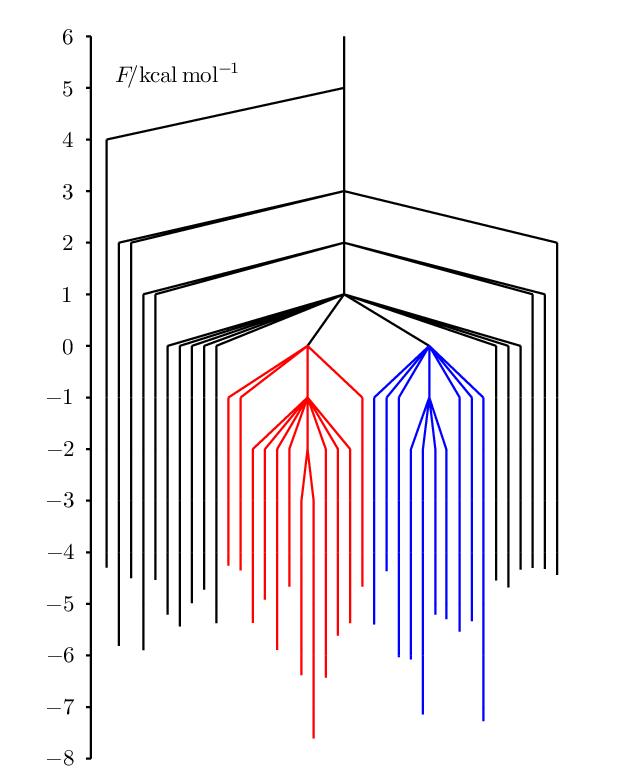
\includegraphics[height=0.75\textheight]{figures/funnels.png}
			\label{fig:funnels}
			\caption{Energy disconnectivity graph for met-enkephalin at 298 K. The low-energy region of the graph contains two funnels, highlighted in red and blue. Source: \cite{Wales2005}}
		\end{figure}
	\end{frame}

	\begin{frame}
		\frametitle{Broken Ergodicity}
		\begin{itemize}
			\item In systems with multiple Funnels, the energy barriers between these funnels can be very high
			\item Monte-Carlo simulations struggle to cross these barriers in the available simulation time
		\end{itemize}
		$\Longrightarrow$ Broken Ergodicity\\
		$\Longrightarrow$ The simulation does not reach every point in configuration space with non-zero probability
	\end{frame}

	\begin{frame}
		\frametitle{Current Methods}
		\begin{itemize}
			\item Parallel Tempering (PT)
			\begin{itemize}
				\item Run at different $T$ in paralell and information is propagated down
				\item Low temperatures of interest necessitate many instances run in paralell $\Rightarrow$ inefficient
			\end{itemize}
			\item Minima Hopping
			\begin{itemize}
				\item Needs prior information about the positions of the local minima
			\end{itemize}
		\end{itemize}
	\end{frame}

	\section{Funnel Hopping Monte Carlo:\\The Method}
	\begin{frame}
	asdf
	\end{frame}
















































\begin{frame}
  	\printbibliography[heading=bibintoc]

  \end{frame}
\end{document}